\section{Introduction}
\label{sec:intro}

With the rapid growth of world population and the loss of arable land, there is an increasing desire to improve the yield and quality of crops, where the understanding of the genetic mechanisms to influence plant growth is a key enabler~\cite{doos2002population}.
%
A classic genetics approach is to produce a diverse population of mutant lines, grow them either in growth chambers with simulated environmental conditions or directly in the field, visually observe the plants during the growth period, and finally identify plant morphological or physiological patterns that tightly associate with key growth factors~\cite{houle2010phenomics}.
%
While many factors can be assessed quantitatively, which is essential for high-throughput study, one of the bottleneck in this research pipeline is plant visual phenotyping~\cite{walter2015plant}.

\begin{figure*}
\begin{centering}
\begin{tabular}{@{}c c c c c}
%\begin{tabular}{lllllllll}
(a) &
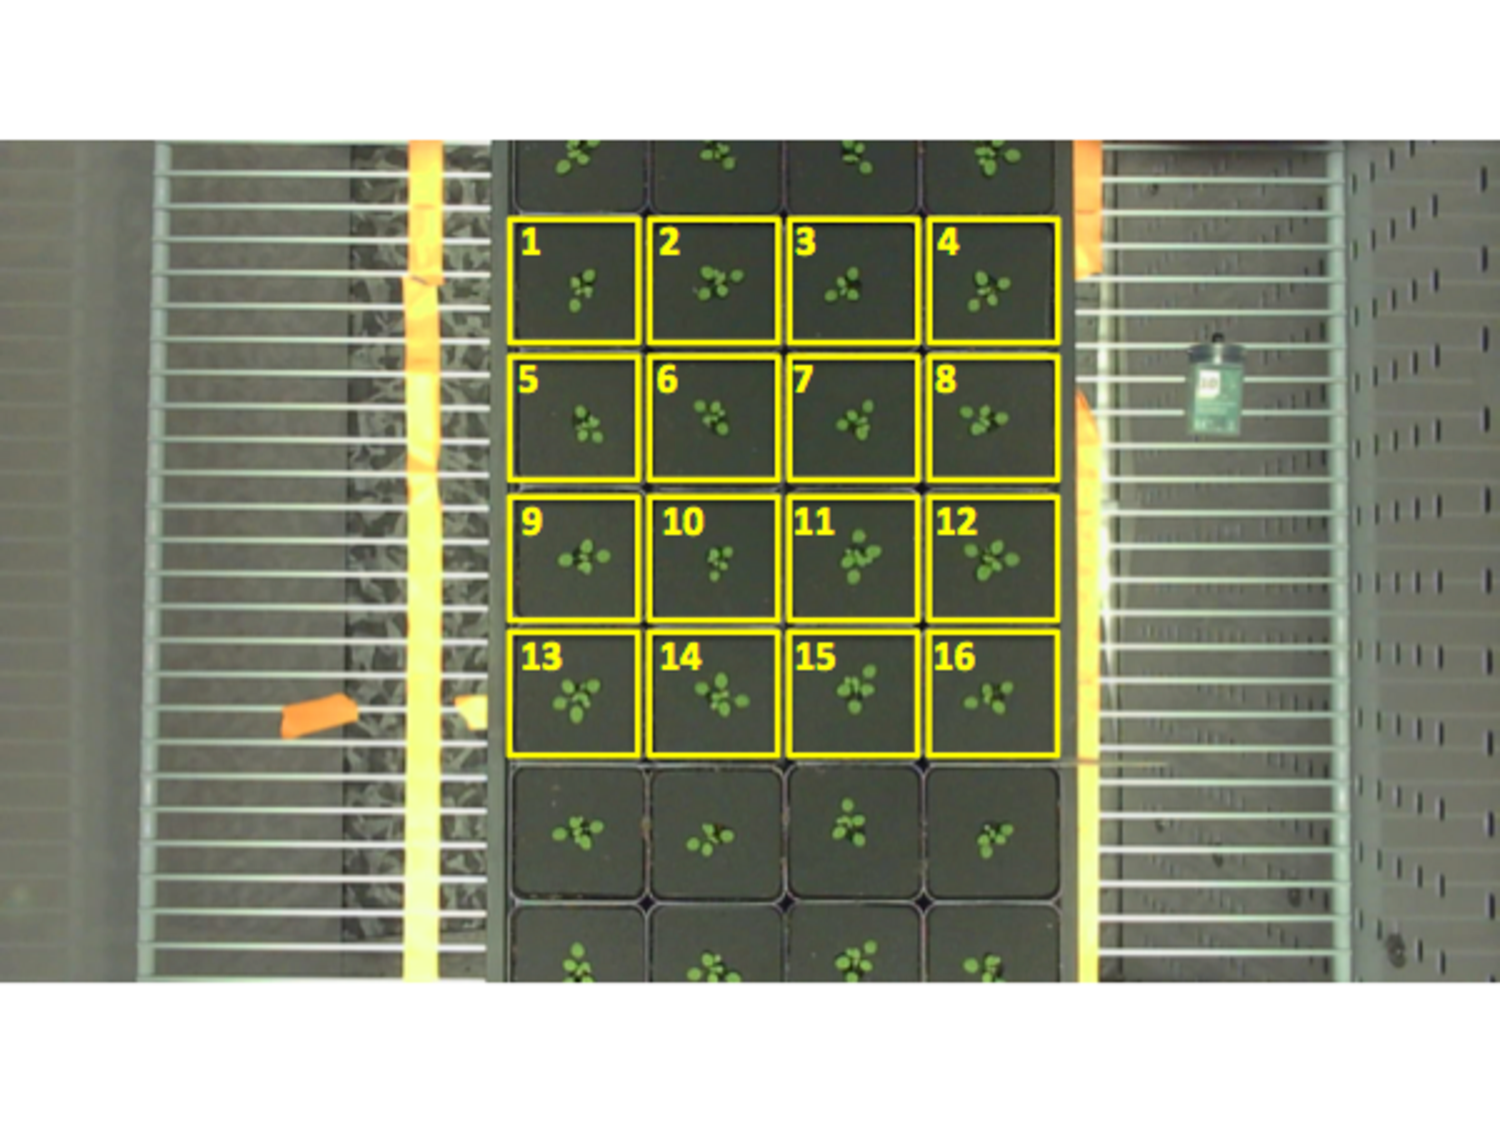
\includegraphics[width=.23\textwidth]{Figures/FourModalities/A_rgb}&
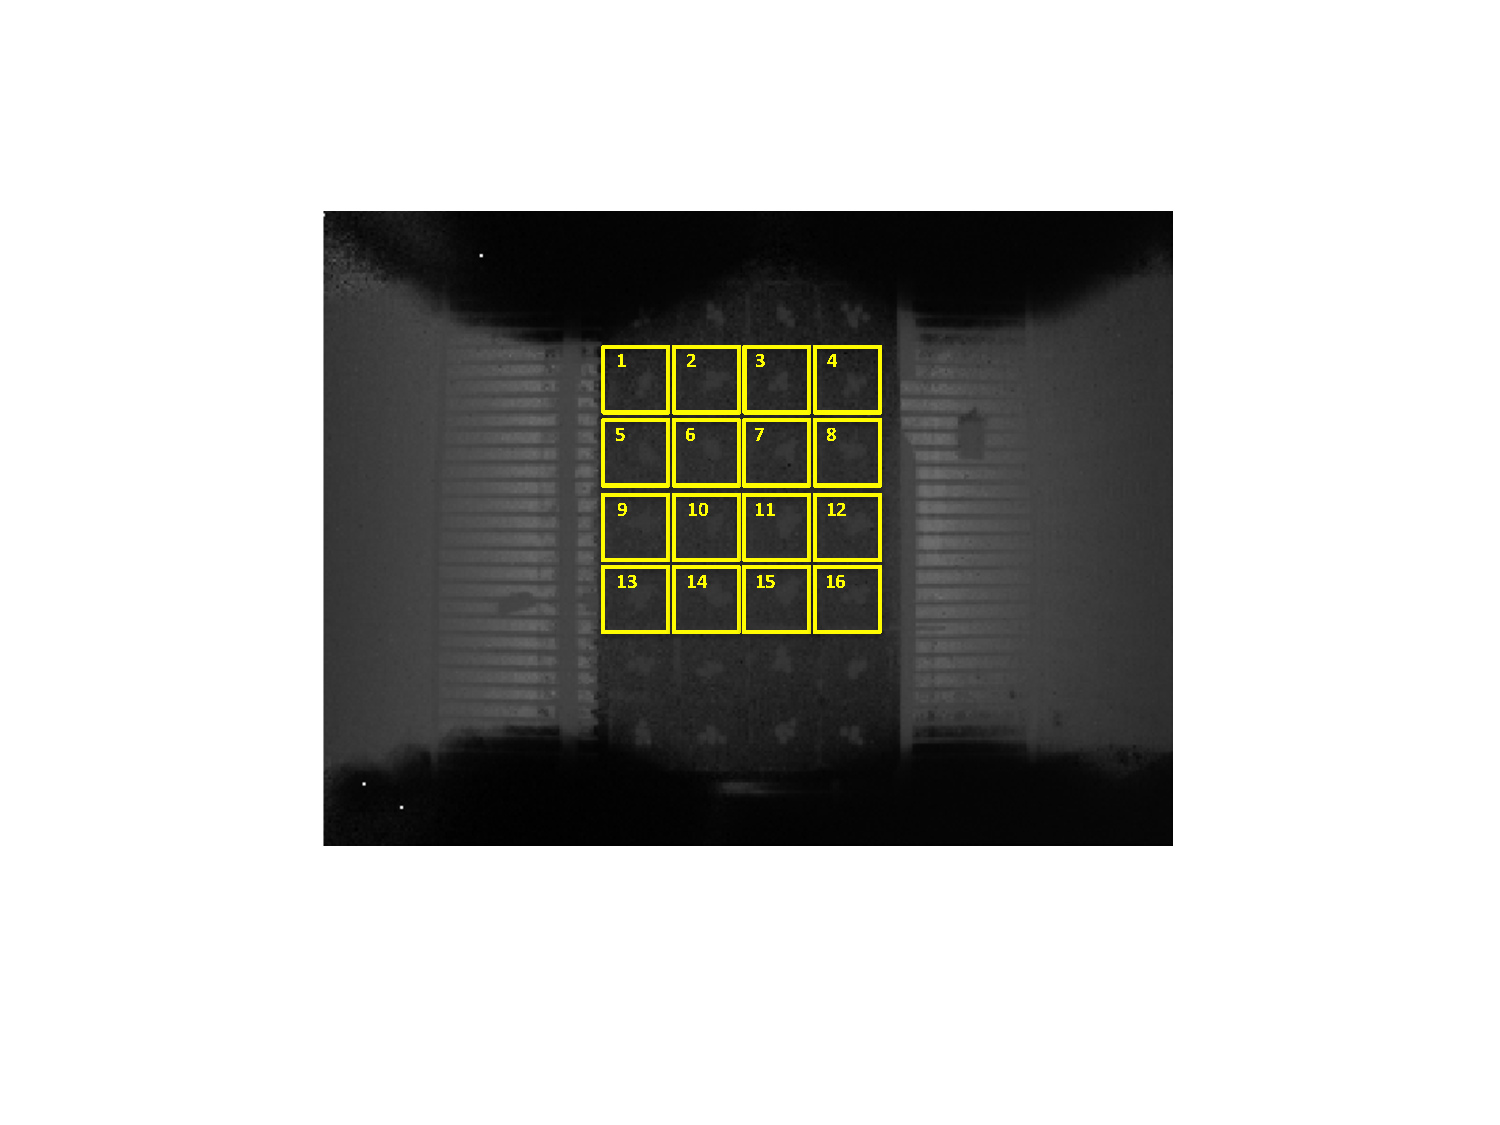
\includegraphics[width=.23\textwidth]{Figures/FourModalities/A_depth}&
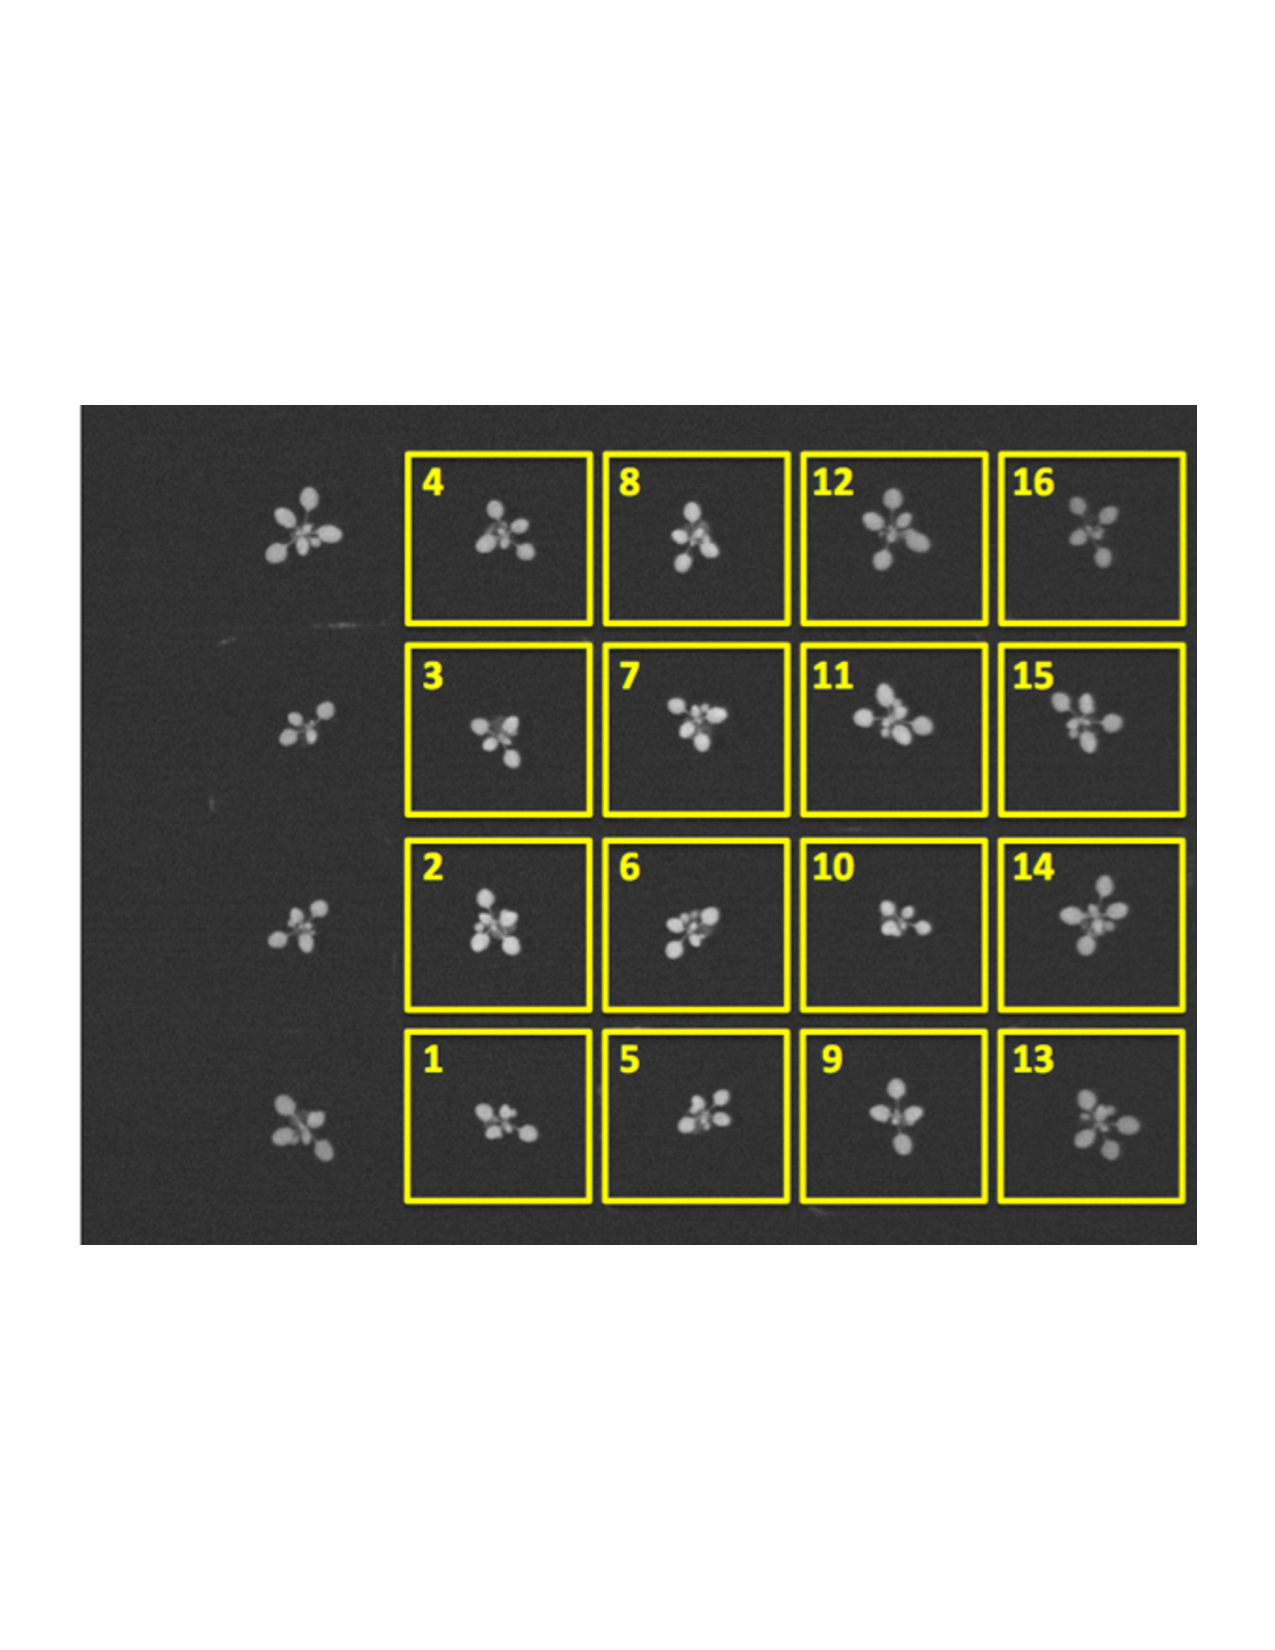
\includegraphics[width=.23\textwidth]{Figures/FourModalities/A_fmp}&
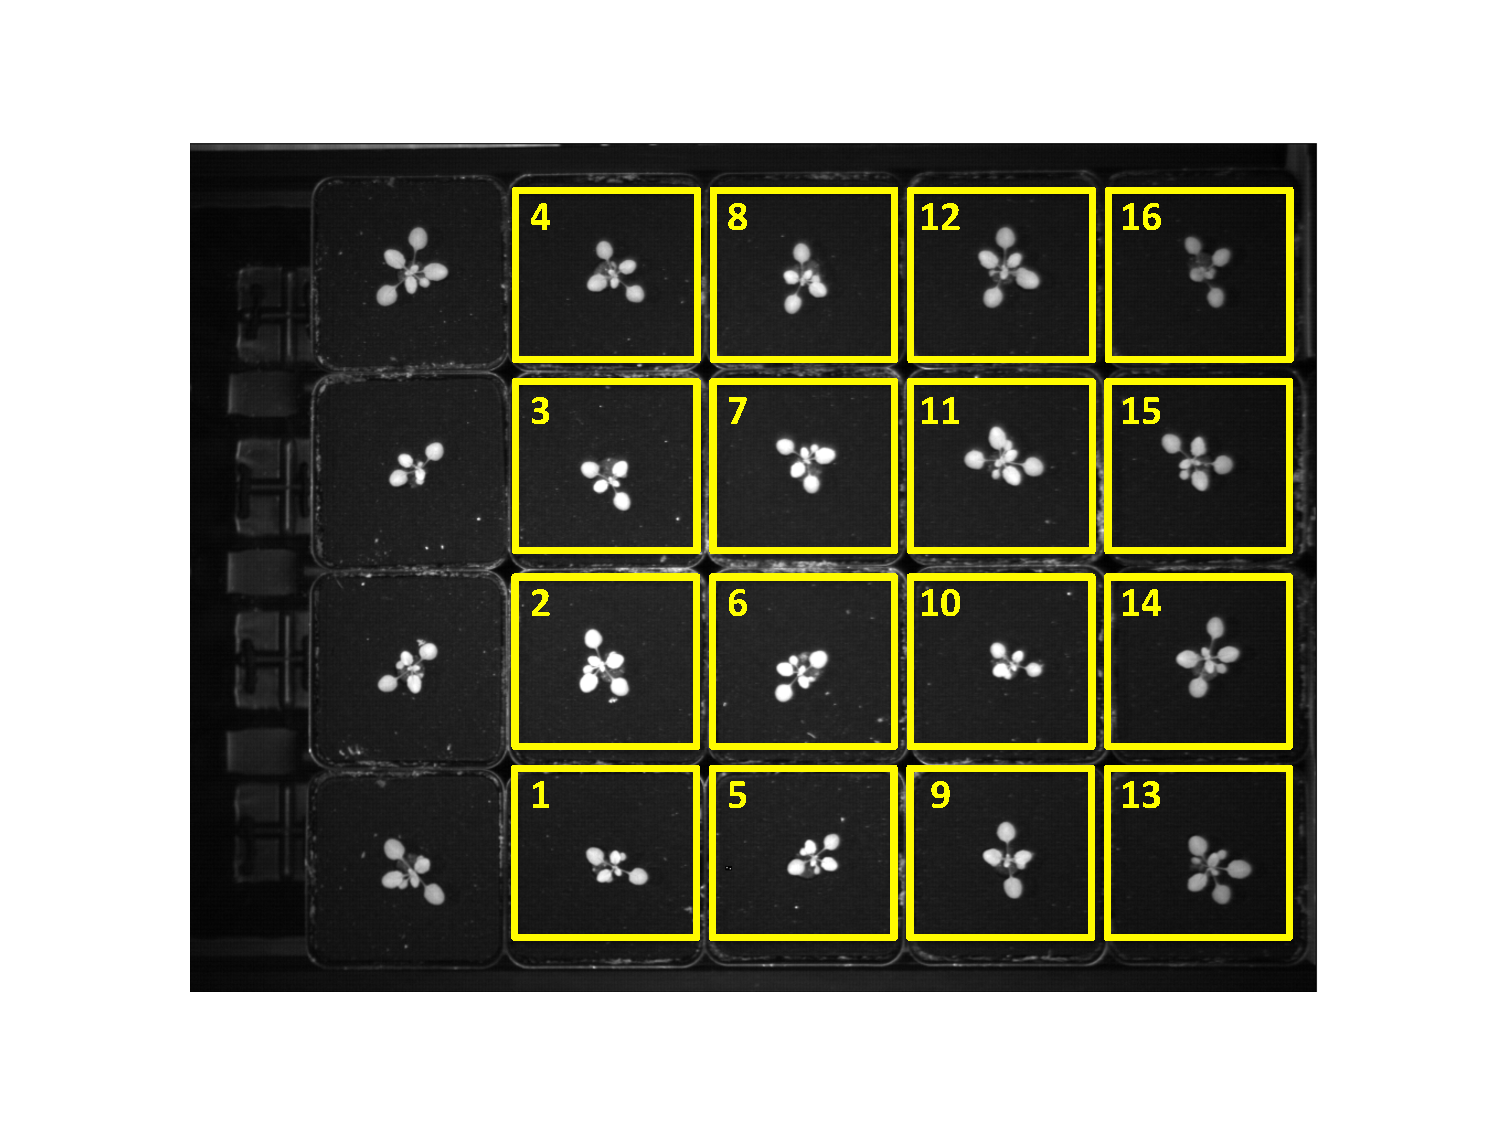
\includegraphics[width=.23\textwidth]{Figures/FourModalities/A_ir}\\
(b) &
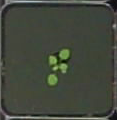
\includegraphics[width=.1\textwidth]{Figures/FourModalities/A1_rgb}&

\includegraphics[width=.1\textwidth]{Figures/FourModalities/A1_depth}&
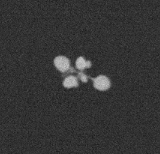
\includegraphics[width=.1\textwidth]{Figures/FourModalities/A1_fmp}&
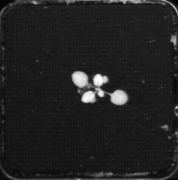
\includegraphics[width=.1\textwidth]{Figures/FourModalities/A1_ir}\\
%Arabidopsis: RGB & Arabidopsis: depth & Arabidopsis: fluorescence & Arabidopsis: IR \\
(c) &
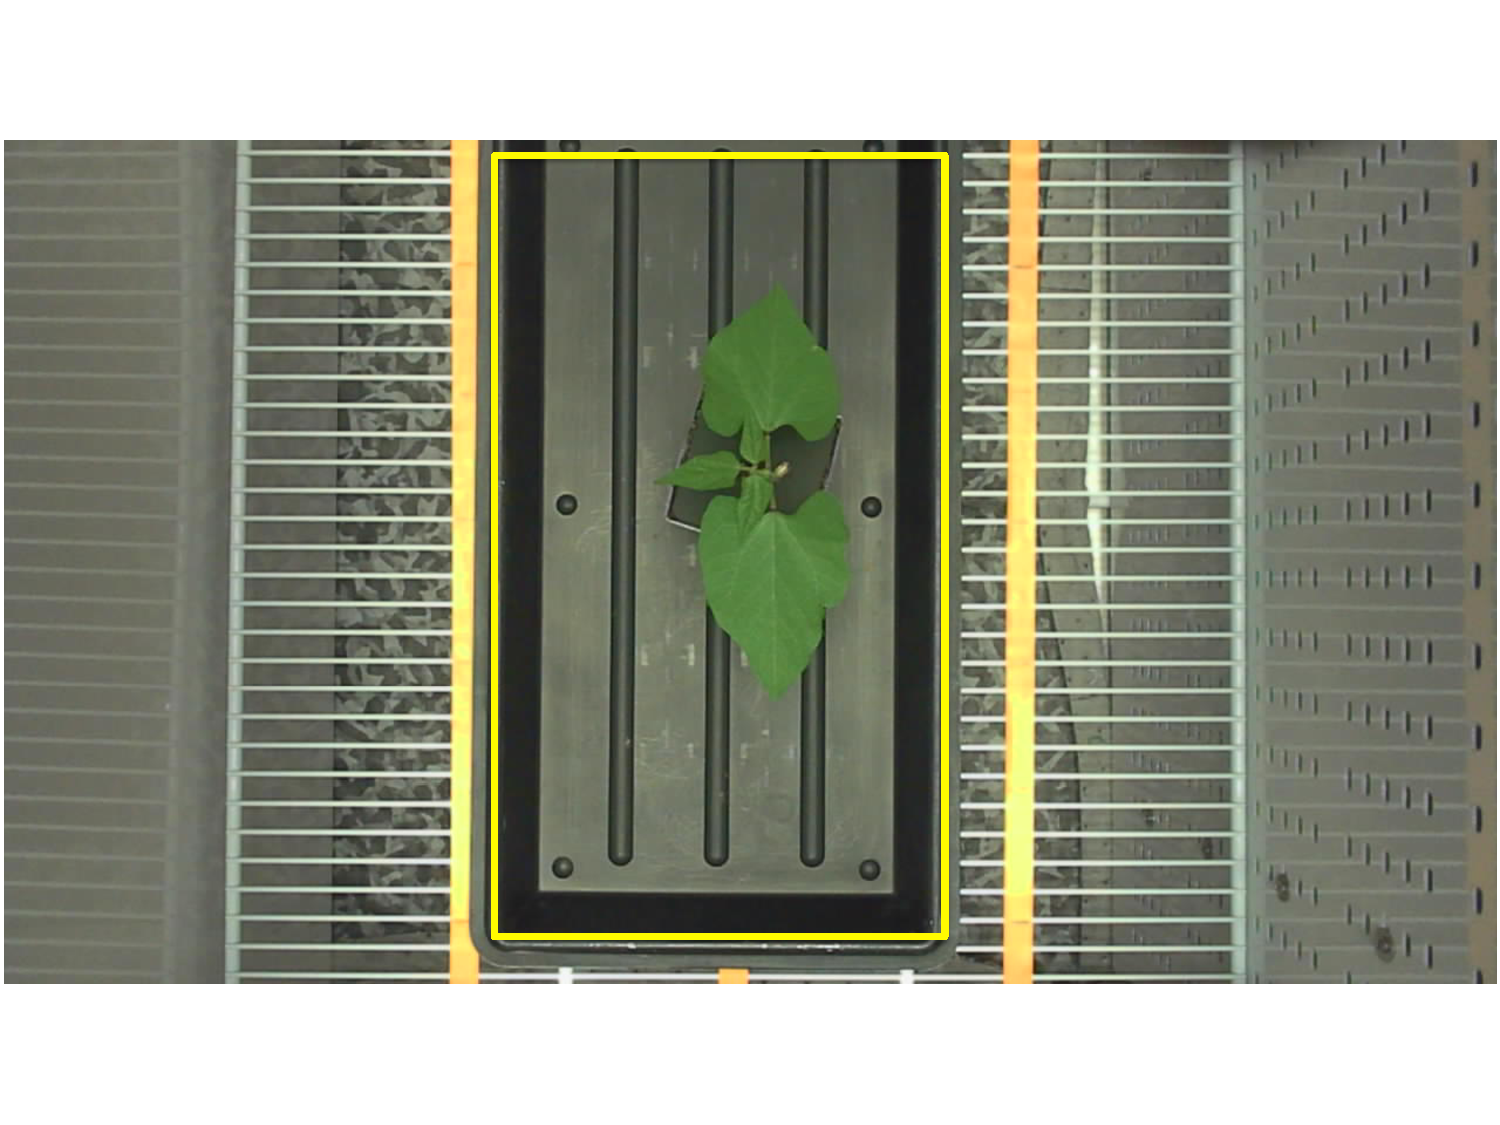
\includegraphics[width=.23\textwidth]{Figures/FourModalities/B_rgb}&
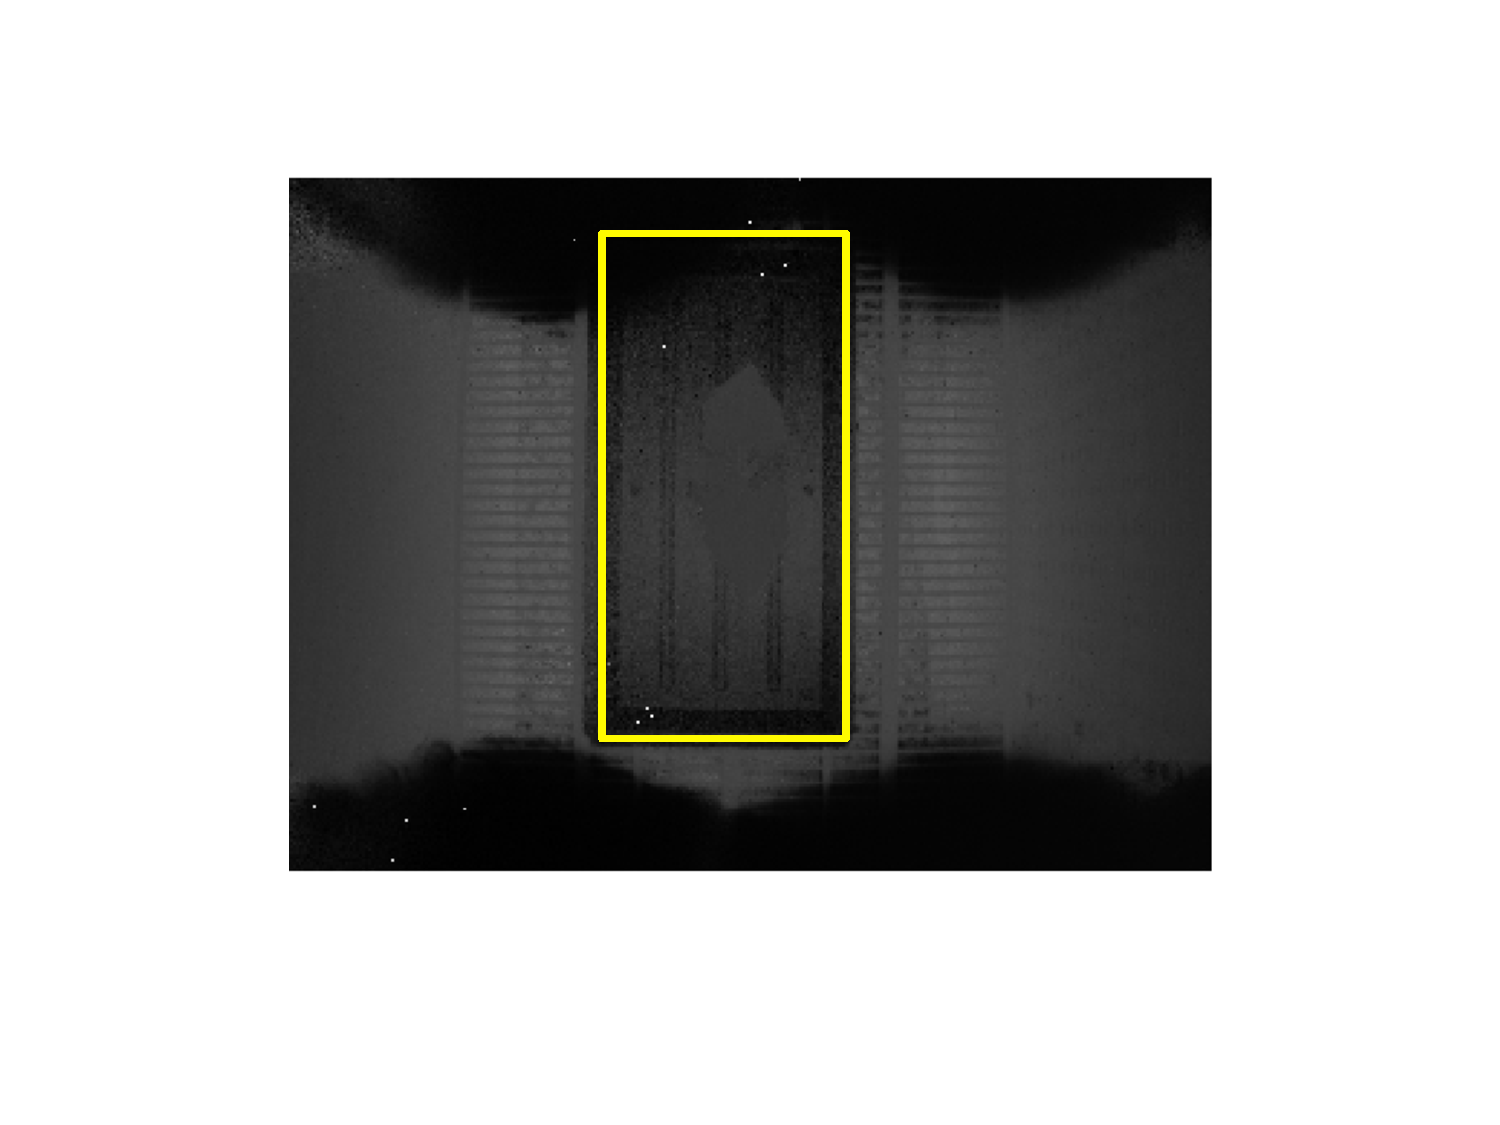
\includegraphics[width=.23\textwidth]{Figures/FourModalities/B_depth}&
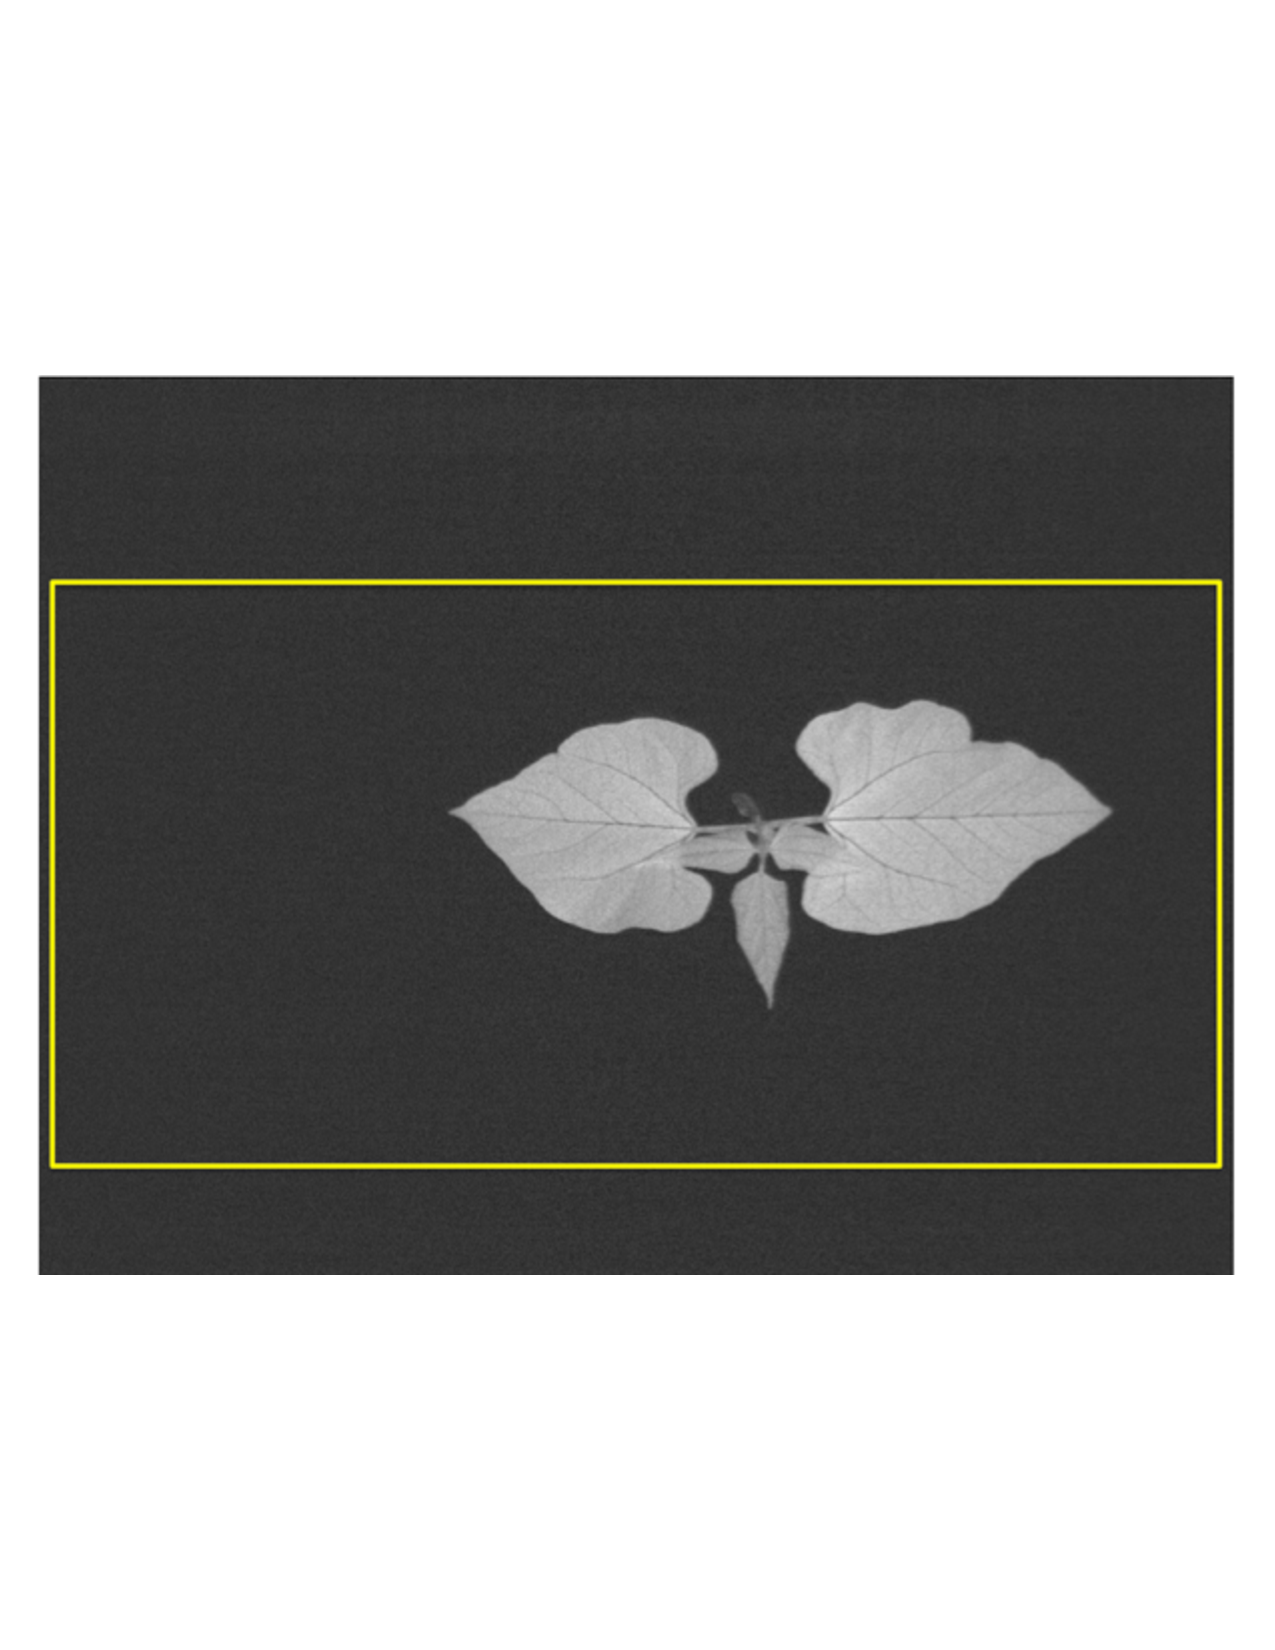
\includegraphics[width=.23\textwidth]{Figures/FourModalities/B_fmp}&
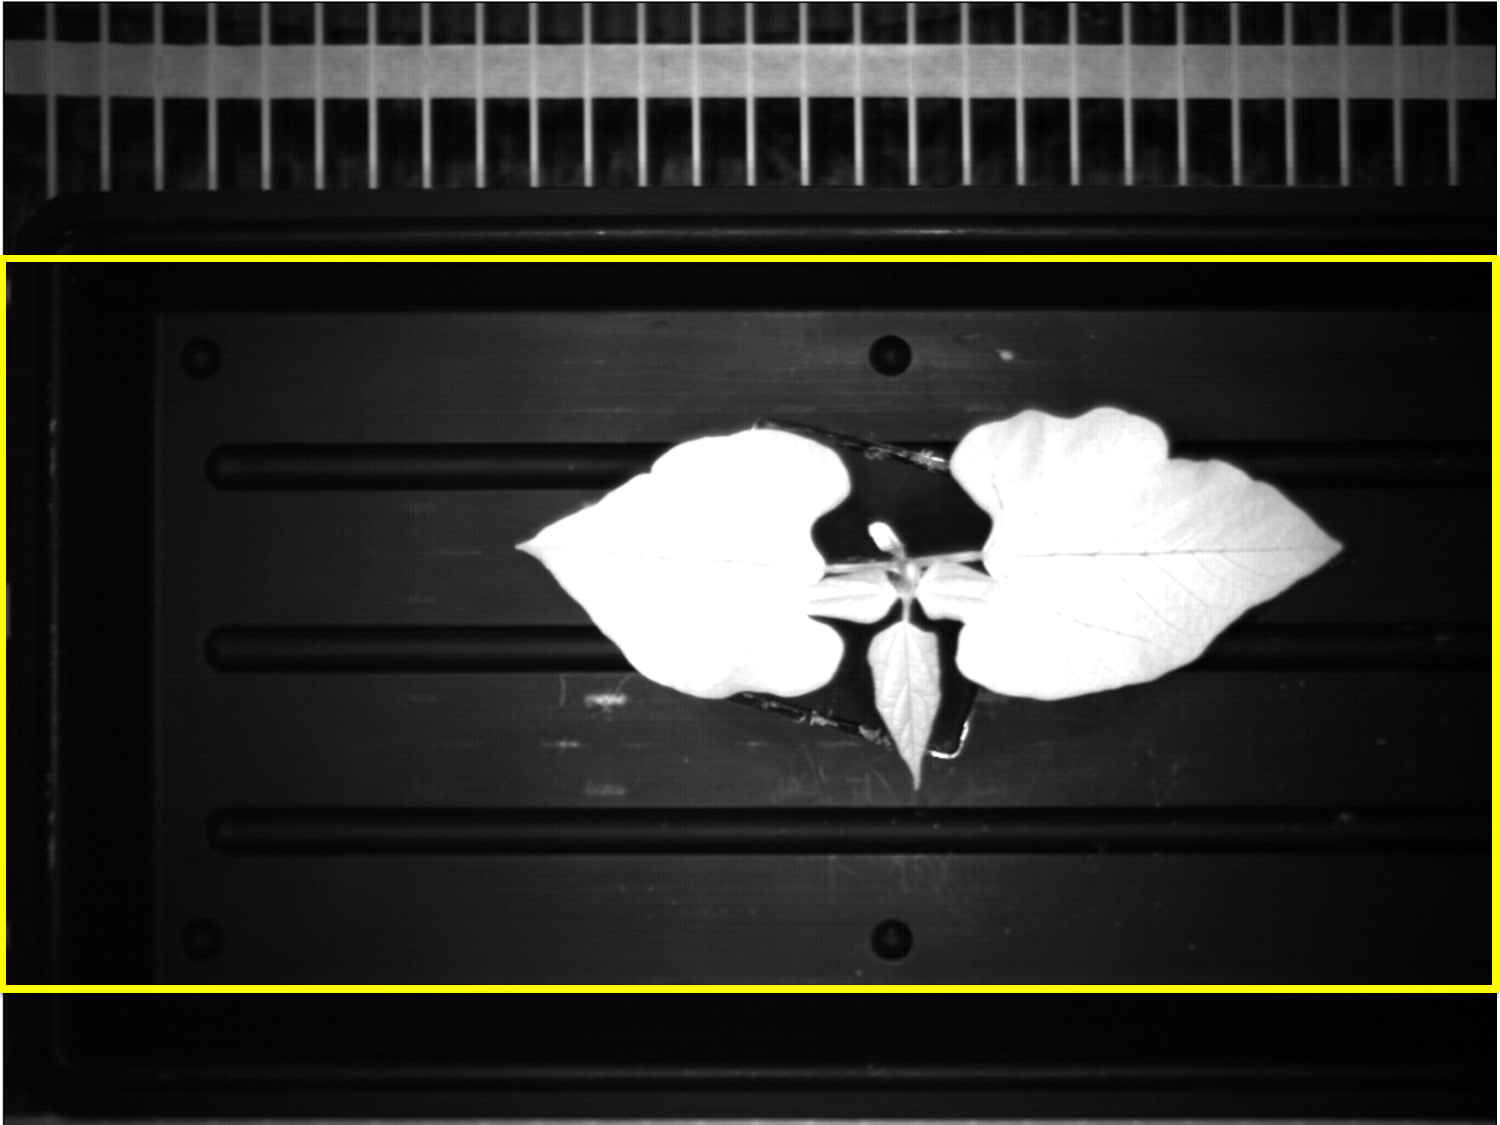
\includegraphics[width=.23\textwidth]{Figures/FourModalities/B_ir}\\
(d) &
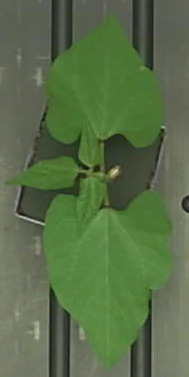
\includegraphics[width=.1\textwidth]{Figures/FourModalities/B1_rgb}&

\includegraphics[width=.1\textwidth]{Figures/FourModalities/B1_depth}&
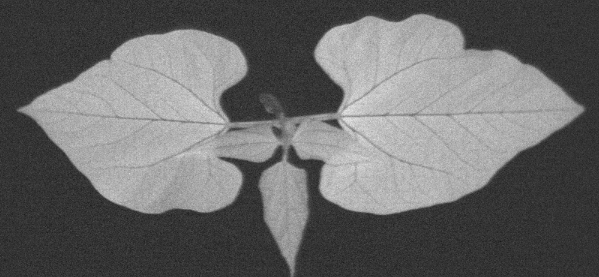
\includegraphics[width=.2\textwidth]{Figures/FourModalities/B1_fmp}&
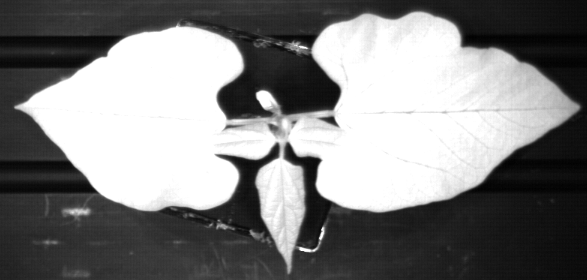
\includegraphics[width=.2\textwidth]{Figures/FourModalities/B1_ir}\\
%Bean: RGB & Bean: depth & Bean: fluorescence & Bean: IR \\
 & RGB & depth & fluorescence & IR\\
\end{tabular}
\caption{The multi-modality plant imagery database of MSU-PID. (a) four modalities of Arabidopsis; (b) zoom in view of Arabidopsis plant $1$; (c) four modalities of bean; (d) zoom in view of bean plant.}
\label{fig:fourmodality}
\end{centering}
\end{figure*}


The objective of {\it plant visual phenotyping} is to analyze and categorize the visual appearance of plants. %~\cite{}.
In old days, plant phenotyping was conducted through manual visual observation~\cite{Erblichkeit1903}.
Today, motivated by the increasing lower cost and increasing diversity of imaging sensors and advances of computer vision technologies, image-based automatic plant visual phenotyping is quickly growing into a desirable and viable solution~\cite{furbank2011phenomics,cruz2015depi}.
In this interdisciplinary field, scientists employ various imaging sensors to capture plants and design advanced algorithms to automatically analyze the captured plant imagery, with the purpose of raising testable biological hypotheses to solve the aforementioned problems.



\begin{table*}[t!]
\centering
\begin{threeparttable}
\caption{Plant image databases.}
%\resizebox{12cm}{!} {
%\begin{tabular}{|l@{}|@{}c@{}|@{}c@{}|@{}c@{}|@{}c@{}|@{}c@{}|}
\begin{tabular}{l|c|c|c|c|c|c}
\hline
\multirow{2}{*}{Database}& \multirow{2}{*}{Modality} & \multirow{2}{*}{Applications}\tnote{a} & \multirow{2}{*}{Plant Type} & Subject/ &Total & Labeled \\
& & & & Classe \# & Image \# & Image \# \\ \hline
Swedish leaf & Scaned leaf & LC& Swedish trees & $15$ & $1,125$ & $1,125$ \\ \hline
Flavia & RGB & LC& Leaves & $32$ & $2,120$ & $2,120$ \\ \hline
Leafsnap & RGB & LC& USA trees & $184$ & $29,107$ & $29,107$ \\ \hline
Crop/weed & RGB &Weed detection & Crop/weed & $2$ & $60$ & $60$ \\ \hline
\multirow{2}{*}{LSC} & \multirow{2}{*}{RGB} & \multirow{2}{*}{LS, LO} & Arabidopsis & $43$ & $6287$ & $201$ \\ \cline{4-7}
& & & Tobacco & $80$ & $165,120$ & $83$ \\ \hline
\multirow{2}{*}{MSU-PID} & fluorescence, & LS, LO, & Arabidopsis & $16$ & $2304\times 4$ & $576\times 4$ \\ \cline{4-7}
& IR, RGB, depth & LA, LT & Bean & $5$ & $350\times 4$ & $175\times 4$ \\ \hline
\hline
\end{tabular}
%}
\begin{tablenotes}
\footnotesize
\item[a] The abbreviation in ``Applications'' column is defined as Leaf Classification (LC), Leaf Segmentation (LS), Leaf Counting (LO), Leaf Alignment (LA), and Leaf Tracking (LT).
\end{tablenotes}
\end{threeparttable}
\label{tab:database}
\end{table*}

Due to diverse variations of leaf shape, appearance, layout, growth and movement, plant image analysis is a non-trivial computer vision task~\cite{Minervini2015}.
In order to develop advanced computer vision algorithms, image databases that are well representative of this application domain is highly important.
In fact, computer vision research lives on and advances with databases, as evidenced by the successful databases in the field (e.g., FERET~\cite{Phillips2000} and LFW~\cite{LFW}).
However, the publicly available database for plant phenotyping is still very limited, with the only exception of LSC database~\cite{scharr2014annotated}, which, nevertheless, has its own limitations on the type of images (RGB only) and is only suitable for a small set of plant image analysis applications.



To facilitate future research on plant image analysis, as well as remedy the limitation of existing databases in the field, this paper presents a newly collected multi-modality Plant Imagery Database through an interdisciplinary effort at Michigan State University (MSU), termed ``MSU-PID''.
As illustrated in Figure~\ref{fig:fourmodality}, the MSU-PID database includes the imagery of two types of plants (Arabidopsis and bean), both are widely used in plant research, captured by four types of imaging sensors, i.e., fluorescence, infrared (IR), RGB color, and depth.
All four sensors are synchronized and are programmed to periodically capture imagery data for multiple consecutive days.
Checkerboard-based camera calibration is performed between a pair of sensors, which results in the explicit correspondence between the pixels of {\it any} two modalities.

The type and amount of manual labels on a database is a critical enabler to the potential applications of the database.
For a subset of the MSU-PID database, we manually label the ground truth regarding the leaf identification number, locations of leaf tips and leaf segments.
As a result, MSU-PID is suitable for a number of applications, including 1) {\it leaf segmentation} that aims at estimating the correct segmentation mask of each leaf in an image, 2) {\it leaf counting} that estimates the correct number of leaves within a plant, 3) {\it leaf alignment} that aligns the two tips of each leaf -- the cornerstone of the leaf structure, and 4) {\it leaf tracking} that is designed to track each leaf over time.
Finally, to provide a performance baseline for future research and comparison, we apply our automatic leaf segmentation framework~\cite{yin2014a,yin2014b} to the Arabidopsis imagery and demonstrate the unique challenge of image analysis on this database.

In summary, this paper and our database have made the following main contributions.
\begin{itemize}
\item MSU-PID is the first {\it multi-modality} plant image database. This allows researchers to study the strength and weakness of individual modality, as well as their various combinations in plant image analysis.
\item Our unique imaging setup and the variety of manual labels make MSU-PID an ideal candidate for evaluating a diverse set of plant image analysis applications, including leaf segmentation, leaf counting, leaf alignment, leaf tracking, and potentially leaf growth prediction and $3$D leaf reconstruction.
\end{itemize}










